$k^2$-tree est une structure de données dense conçue à l'origine pour la compression des graphes du web. L'algorithme de base a été proposé par Bisaboa et al. dans leur article \textit{$k^2$-trees for Compact Web Graph} \citep{brisaboa2009k}. Elle a été appliquée ensuite dans d'autres travaux de compression comme les réseaux sociaux \citep{shi2012optimizing}, les données rasters \citep{de2013compact} et les bases de données \gls{rdf} \citep{alvarez2017succinct}.\\

En général, l'algorithme peut être appliqué à n'importe quelle matrice binaire. Dans le cadre de notre étude nous nous intéressons seulement à la matrice d'adjacence d'un graphe.
La compression par les $k^2$-trees exploite les propriétés de la matrice d'adjacence et tire parti des zones vides pour réduire l'espace de stockage et permettre au graphe de tenir en mémoire centrale. Il offre aussi la possibilité de naviguer dans le graphe sans le décompresser, et de répondre aux requêtes de voisinage direct et inverse.

Étant donné une matrice d'adjacence A d'ordre $|n|$, $k^2$-tree la représente sous forme d'un arbre de recherche $k^2$-aires \footnote{Les arbres n-aires sont une généralisation des arbres binaires : chaque nœud a au plus n fils.} de hauteur h = [$log_{k}$ n]. Chaque nœud de l'arbre contient un seul bit avec deux valeurs possibles : 1 pour les nœuds internes et 0 pour les feuilles, sauf le dernier niveau où les feuilles représentent les cases de la matrice A et peuvent prendre une valeur 0 ou 1. Chaque nœud interne de l'arbre a exactement $k^2$ fils.  
Avant la construction de l'arbre, il faut s'assurer que n est une puissance de k. Dans le cas contraire, l'algorithme étend la matrice en rajoutant des zéros à droite et en bas de la matrice. L'ordre de la matrice devient donc $n'= k^{log_{k} n}$.\\

Pour construire l'arbre, $k^2$-tree commence par diviser la matrice en $k^{2}$ sous matrices d'ordre $|n/k|$. La racine correspond à la matrice complète. Chaque sous matrice représente un nœud dans le premier niveau de l'arbre, elle est ajoutée comme un fils à la racine suivant un ordre de gauche à droite et de haut en bas. Le nœud est à 1 si la sous matrice qu'il représente contient au moins un 1, et à 0 si elle ne contient que des 0. Le processus est répété de manière récursive sur les sous matrices représentées par des 1. $k^{2}$ sous matrices sont considérées à chaque subdivision. L'opération est répétée jusqu'à ce que la subdivision atteint les cases de la matrice qui représenterons les feuilles de l'arbre au dernier niveau. 

La figure \ref{k2-trees-exemples} illustre la représentation $k^2$-tree d'une matrice de taille $10 \times 10$, étendue à une  taille $16 \times 16$ pour un k=2 \citep{brisaboa2015efficient}.

\begin{figure}[H]
\begin{center}
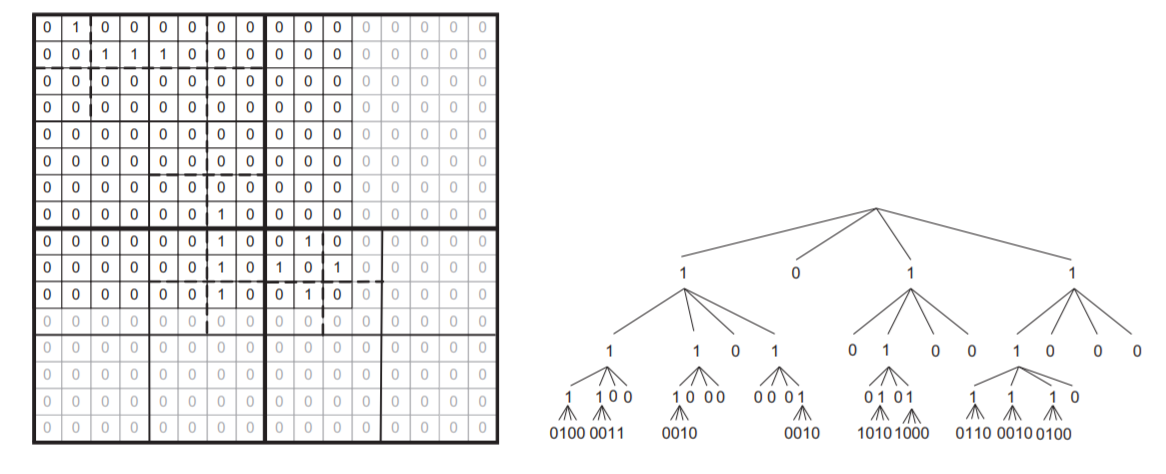
\includegraphics[height=200 pt, width=450 pt]{./ressources/image/k2-trees.png} 
\end{center}
\caption{Exemple de représentation $k^2$-tree}
\label{k2-trees-exemples}
\end{figure}


Pour le stockage de l'arbre, l'algorithme utilise deux tableaux binaires : un tableau T (Tree) contenant tous les nœuds de l'arbre à l'exception du dernier niveau et un tableau L (Leaves) contenant les feuilles du dernier niveau. Les nœuds et les feuilles sont ordonnés selon un parcours en largeur de l'arbre.   
Ci-dessous les deux tableaux T et L de l'exemple précédent (figure \ref{k2-trees-exemples}) : \\
\begin{center}
	T = 1011 1101 0100 1000 1100 1000 0001 0101 1110\\
	L = 0100 0011 0010 0010 1010 1000 0110 0010 0100\\	
\end{center}
Dans le pire des cas, l'espace total pour la description de la structure est $k^2*m(log_{k^2}\frac{n^2}{m}+ \textit{O}(1))$, où n est le nombre de nœuds du graphe et m le nombre de liens. Cependant, pour les graphes réels, l'espace nécessaire pour le stockage est bien meilleur. \\

Dans le même article \citep{brisaboa2009k}, et dans le but d'obtenir un compromis entre la taille de l'arbre et le temps de parcours, les auteurs proposent une hybridation qui consiste à changer la valeur du paramètre k en fonction du niveau de l'arbre en donnant à k une grande valeur au début pour réduire le nombre de niveaux et améliorer ainsi le temps de recherche, et une petite valeur à la fin pour avoir des petites sous matrices et réduire l'espace de stockage.
Pour le stockage de l'arbre, un tableau $T_{i}$ est utilisé pour chaque valeur $k_{i}$, le tableau L reste le même.\\

Plusieurs variantes de l'algorithme de base ont été proposées dans la littérature dont le but était soit d'obtenir un meilleur résultat de compression, soit d'appliquer la méthode sur d'autres types de graphes. Nous allons dans ce qui suit présenter les principaux travaux qui traitent ce sujet.\\

Dans \citep{shi2012optimizing}, les auteurs proposent deux techniques d'optimisation de l'algorithme : la première consiste à trouver un certain ordre des nœuds qui permet de regrouper les 1 de la matrice d'adjacence dans une seule sous matrice au lieu qu'ils soient dispersés de manière aléatoire. La recherche d'un ordre optimal des nœuds n'est pas envisageable. Avec k=2,le problème peut être réduit à un autre problème (min bisection\footnote{Le problème de bissection minimale (MBP) est un problème NP-hard bien connu, qui est destiné à diviser les sommets d'un graphe en deux moitiés égales afin de minimiser le nombre de ces arêtes avec exactement une extrémité dans chaque moitié.}) qui est NP-difficile. Les auteurs utilisent alors un parcourt \newacronym{dfs}{DFS}{Deapth First Search}\gls{dfs}
\footnote{\gls{dfs} : Parcours en profondeurs du graphe}
 avec des heuristiques pour trouver une approximation de l'ordre optimal. Cette optimisation permet de réduire le nombre de nœuds internes et produit ainsi un arbre optimal. La deuxième optimisation est de trouver la valeur de k la plus adéquate pour chaque nœud interne, calculer cette valeur pour chaque nœud peut engendrer un temps de calcul très important. Pour éviter cela, les auteurs affectent la même valeur k pour les nœuds ayant le même parent. 	

Dans un travail ultérieur \citep{brisaboa2014compact}, les auteurs de l'article de base apportent deux améliorations principales de leur méthode dans le but d'optimiser l'espace et le temps de parcours de l'arbre produit. La première est de construire $k^2$ arbres distincts pour les $k_{0}^{2}$ sous matrices du premier niveau. Elle présente plusieurs avantages : (1) l'espace est réduit étant donné que la taille de chaque arbre est en fonction de $\frac{n^2}{k^2}$, (2) le temps de parcours s'améliore puisque T et L sont plus petits. La deuxième amélioration est la compression de L qui consiste à construire un vocabulaire \textit{V} de toutes les sous matrices du dernier niveau sous forme de séquences de bits, les classer par fréquence d'apparition et remplacer leurs occurrences dans L par des pointeurs. Cela permet d'éviter la redondance et de réduire la taille de la structure. Les pointeurs sont représentés par des codes de longueur variable ordonnés, le plus petit correspond à la sous matrice la plus fréquente. Néanmoins, cette représentation ne permet pas un accès direct dans L étant donné qu'une décompression séquentielle est nécessaire pour récupérer une position. Pour remédier à ce problème, les auteurs utilisent le principe de
\newacronym{dac}{DAC}{Directly Addressable Codes}
 \gls{dac}\footnote{\gls{dac} est une technique qui encode une séquence d'entiers ou mots en utilisant une structure à longueur variable, son avantage principale est l'accès direct au mot sans passer par le décodage.} \citep{brisaboa2013dacs} pour garantir un accès rapide au pointeur et conserver ainsi une navigation efficace.\\
Exemple : Pour la figure \ref{k2-trees-exemples}, le vocabulaire et L sont représentés comme suit :\\
\begin{center}
\textit{V}= [0010 0100 0011 1010 1000 0110]\\
L = $c_{1}c_{2}c_{0}c_{0}c_{3}c_{4}c_{5}c_{0}c_{1}$ \\
\end{center}

%\subsubsection{d$k^2$-trees}
Dans \citep{brisaboa2012compressed}, les même auteurs développent la représentation $k^2$-trees pour les graphes dynamiques. Ils proposent une nouvelle structure nommée d$k^2$-trees pour \textit{Dynamique $k^2$-trees} qui offre les même capacités de compression et fonctionnalités de navigation que le cas statique et qui permet également d'avoir des mises à jour sur le graphe. Pour atteindre ces objectifs, d$k^2$-tree remplace la structure statique de $k^2$-tree par une implémentation dynamique. Dans cette nouvelle implémentation, les deux tableaux T et L sont remplacés par deux arbres, nommés $T_{tree}$ et $L_{tree}$ respectivement. Les feuilles de $T_{tree}$ et $L_{tree}$ stockent des parties des bitmaps T et L. La taille de ces feuilles est une valeur paramétrable. Les nœuds internes des deux arbres permettent d'accéder aux feuilles et de les modifier.
Chaque nœud interne de $T_{tree}$ contient trois(03) éléments : deux compteurs b et o, qui contiennent respectivement le nombre de bits et le nombre de "1" stockés dans les feuilles descendantes de ce nœud, et un pointeur P vers le nœud fils. Les nœuds internes de $L_{trees}$ sont similaires sauf qu'ils ne contiennent que b et P. Avec cette structuration, $T_{tree}$ et $L_{tree}$ permettent l'ajout et la suppression des liens dans le graphe.\\
La figure \ref{dk2-trees} présente une représentation d$k^2$-tree \citep{brisaboa2012compressed}: 
\begin{figure}[H]
\begin{center}
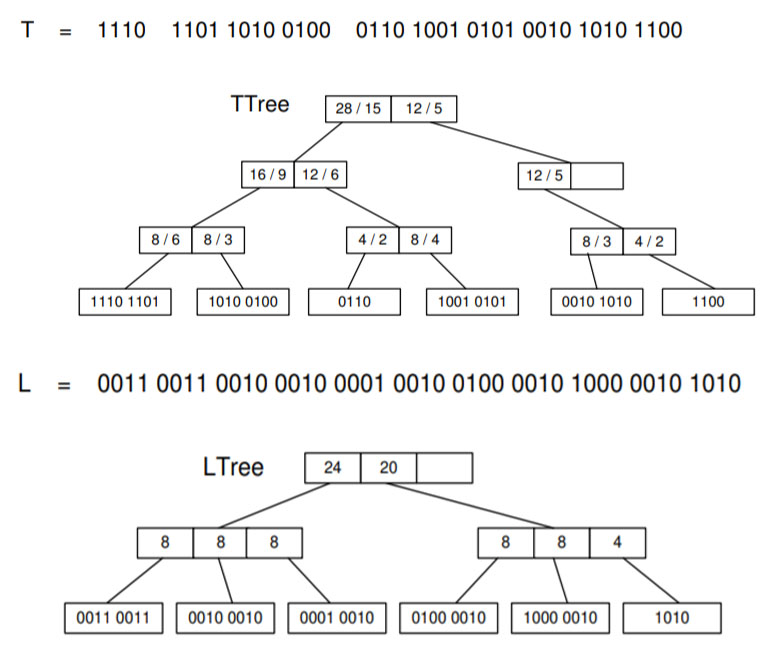
\includegraphics[scale=0.7]{./ressources/image/dk2-trees.jpg} 
\end{center}
\caption{Exemple d'une représentation d$k^2$-tree}
\label{dk2-trees}
\end{figure}

%\subsubsection{$k^n$-trees}
 Sandra et al. \citep{de2013compact} présentent $k^n$-tree, une généralisation des $k^2$-tree pour les problèmes multidimensionnels. Cette méthode possède plusieurs applications. Elle est utilisée pour représenter les bases de données multidimensionnelles, les données rasters et les graphes dynamiques. $k^n$-tree repose sur $k^2$-tree pour représenter une matrice à n-dimensions (dites \textit{tensor} en Anglais). La matrice est décomposé en $k^n$ sous-matrices de même taille, comme suit : sur chaque dimension, K-1 hyperplans devisent la matrice dans les positions i*$\frac{n}{K}$,pour $i \in [1, K-1]$. Une fois les dimensions partitionnées, $k^n$ sous-matrices sont induites, elles sont représentées par des nœuds dans l'arbre comme dans l'algorithme de base. Les structures utilisées pour le stockage sont aussi les mêmes (T et L).
En posant n=3, la méthode peut être appliquée sur les graphes dynamiques ou temporels. Ce type de graphe est représenté par une grille à 3 dimensions $X \times Y \times T$, où les deux premières dimensions représentent les nœuds de départ et de destination, et la troisième dimension représente le temps. 
La figure \ref{kn-trees} présente une représentation $k^3$-tree d'un graphe dynamique \citep{de2014new}.

\begin{figure}[H]
\begin{center}
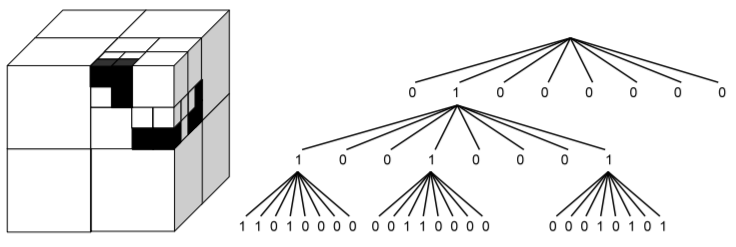
\includegraphics[height=100 pt, width=380 pt]{./ressources/image/kn-trees.png} 
\end{center}
\caption{Exemple d'une représentation $k^3$-tree}
\label{kn-trees}
\end{figure}



%\subsubsection{$K^2$-tress1 }
La représentation de base des arbres k2-trees regroupe seulement les zones de zéros, puisqu'elle a été conçue au début pour les graphes du web qui possèdent une matrice d'adjacence extrêmement creuse. Dans \citep{de2014new}, Les auteurs proposent d'étendre cette représentation en regroupant les zones de "1" également. L'idée générale est d'arrêter la décomposition de la matrice d'adjacence quand une zone unie est trouvée, à savoir des zéros ou des uns. Pour distinguer entre les différents nœuds, une représentation quadtree est utilisée \citep{de1997computational}. Une couleur est attribuée à chaque nœud, blanc pour une zone de zéro, noir pour une zone de uns et gris pour les nœuds internes, i.e, les zones contenant des uns et des zéros. Pour le stockage des nœuds, les auteurs proposent quatre encodages présentés dans ce qui suit : 

\begin{enumerate}[label=$\bullet$]
\item \textbf{ $k^2$-$trees1^{2-bits-naive}$ :} Dans cet encodage, deux bits sont utilisés pour représenter chaque type de nœud. L'attribution des bits n'est pas arbitraire, le premier bit du poids fort indique si le nœud est un nœud interne (0) ou une feuille (1), le deuxième détermine si les feuilles sont blanches (0) ou noires (1). Nous aurons donc : "10" pour les nœuds gris, "01" pour les nœuds noirs et "00" pour les nœuds blancs. Notant que les feuilles du dernier niveau sont représentées par un seul bit.
Après le codage, le premier bit de chaque nœud sauf ceux du dernier niveau est stocké dans T, un autre tableau $T'$ est créé pour sauvegarder le deuxième bit. Les nœuds du dernier niveau sont stockés dans L.
\item \textbf{ $k^2$-$tree1^{2-bits}$ :} Le même principe que l'encodage précédant sauf que les nœuds gris sont représentés par un seul bit, toujours à "1". Le tableau $T'$ va contenir dans ce cas la couleur des feuilles ce qui va réduire la taille de la structure.

\item \textbf{ $k^2$-$tree1^{DF}$ :} Cet encodage est similaire à $k^2$-$trees1^{2-bits}$, mais il utilise un seul bit pour les nœuds blancs et deux bits pour les nœuds noirs et gris, compte tenue de la fréquence des nœuds blancs dans les graphes du monde réel par rapport aux autres. Nous aurons donc : "0" pour les nœuds blancs, "10" pour les nœuds gris et "11" pour les nœuds noirs.

\item \textbf{ $k^2$-$tree1^{5-bits}$ :} Le dernier encodage repose sur la représentation de base. Un nœud blanc est représenté par "0", un nœud noir ou gris par "1", exactement comme le $k^2$-tree d'origine. Pour identifier un nœud noir (zone de uns), il sera représenté par une combinaison impossible : $k^2$ fils de "0" sont ajoutés aux nœuds noirs pour les distinguer.
\end{enumerate}


La figure \ref{k2-trees1-exemple} illustre une représentation $k^2$-tress1 avec les quatre encodages \citep{de2014new} : 


\begin{figure}[H]
\begin{center}
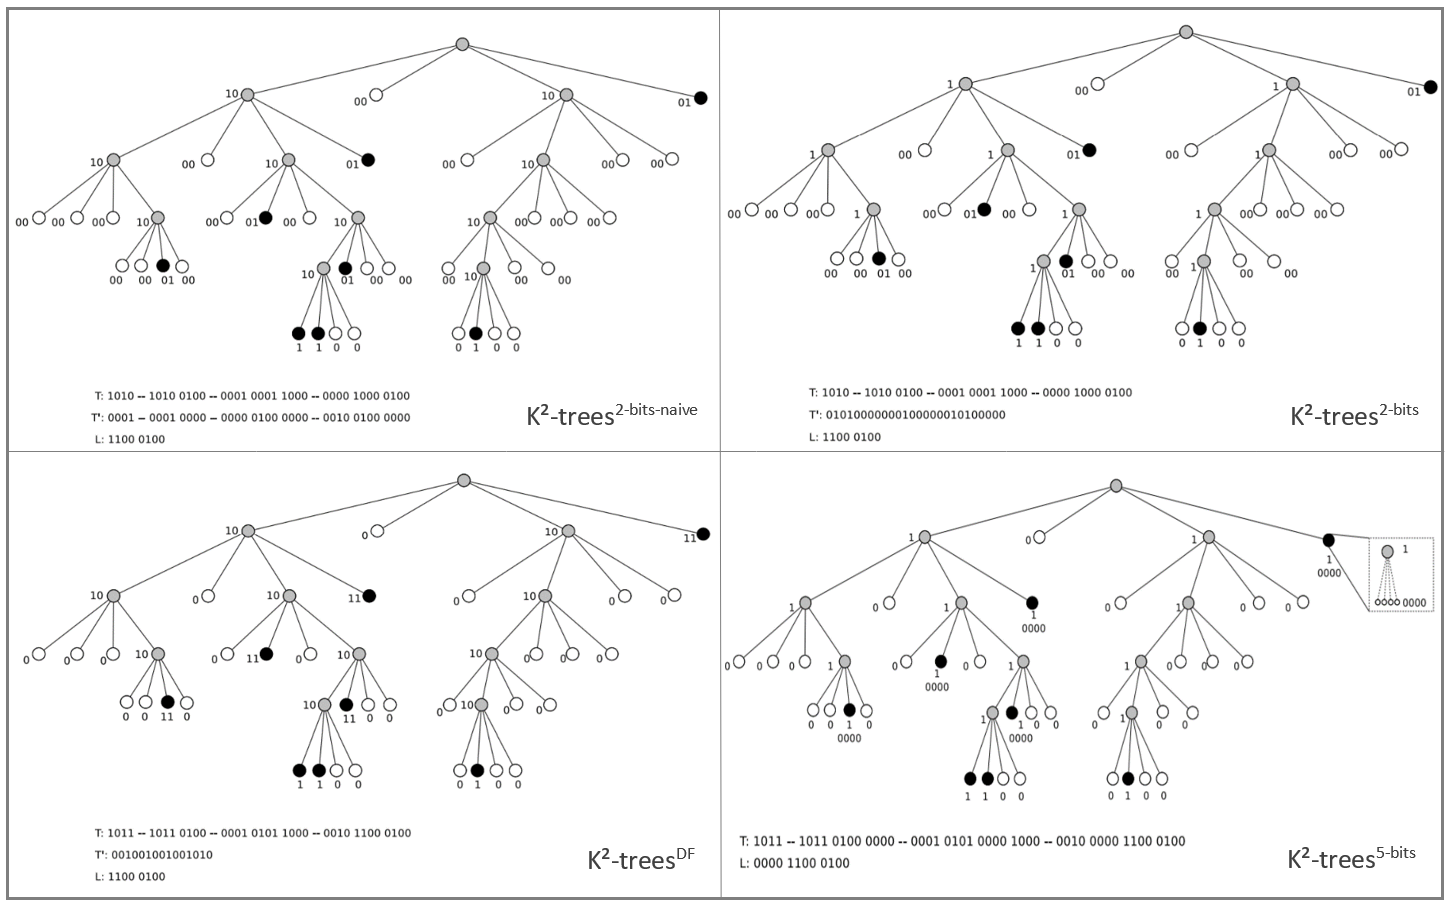
\includegraphics[height=300 pt, width=450 pt]{./ressources/image/k2-trees1.png} 
\end{center}
\caption{Exemple d'une représentation $k^2$-tree1 avec les quatre encodages}
\label{k2-trees1-exemple}
\end{figure}


%\subsubsection{Delta-$K^2$-tress }

Dans \citep{zhang2014delta}, les auteurs proposent Delta-$k^2$-tree, une variante qui exploite la propriété de similarité entre les nœuds voisins du graphe pour réduire le nombre de uns dans la matrice d'adjacence. Notons par \textit{Matrix} la matrice d'adjacence, Delta-$k^2$-trees construit une nouvelle matrice appelée \textit{Delta-matrix}, une ligne \textit{i} de \textit{Delta-matrix} va contenir la différence entre les deux lignes \textit{Matrix}[i] et  \textit{Matrix}[i-1] si cela décroit le nombre de uns sinon elle sera égale à \textit{Matrix}[i], comme suit: \\

$\left\{
\begin{array}{llcl}
\textbf{Si}\ \ count1s(matrix[i]) < countDif(matrice[i],matrix[i-1])\\
\ \ \ \ Delta-matrix[i]  := matrix[i]  \\
\textbf{Sinon} & & &\\
\ \ \ \ Delta-matrix[i]  := matrix[i] \bigoplus matrix[i-1] & 
\end{array}
\right.$\\

Où \textit{count1s} compte le nombre de 1 dans une ligne, \textit{countDif} compte le nombre de bits différents entre deux lignes et $\bigoplus$ représente le "ou exclusif".

Pour déterminer si une ligne est identique à celle de la matrice d'adjacence ou non, un tableau D est utilisé : Si D[i]=1 la ligne est identique, sinon c'est une ligne de différence.\\
La matrice \textit{Delta-matrix} contient moins de uns que la matrice d'adjacence, d'où elle est plus creuse, ce qui permet de réduire la taille de la structure et avoir un meilleur taux de compression. Cependant le temps de parcours est plus grand car pour accéder à certaines lignes (lignes de différence), le graphe doit être décompressé et la matrice d'adjacence reconstituée.\\
La figure \ref{k2-trees-delta} présente un exemple de la représentation Delta-$k^2$-tree \citep{zhang2014delta}.


\begin{figure}[H]
\begin{center}
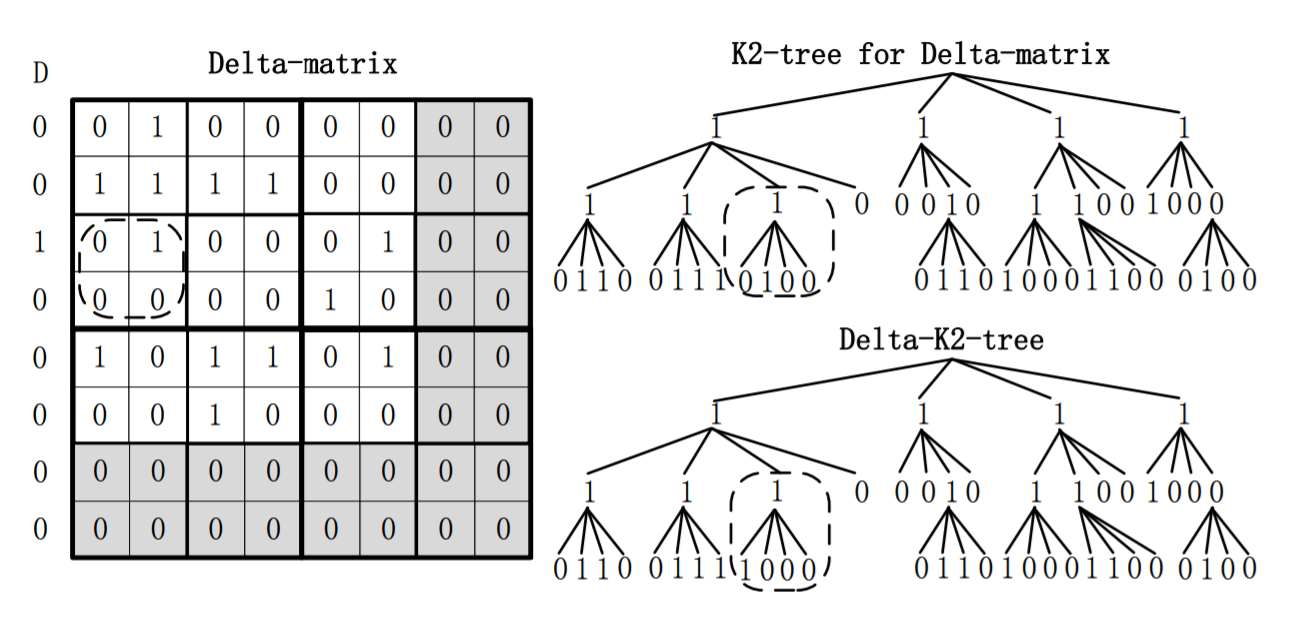
\includegraphics[height=150 pt, width=380 pt]{./ressources/image/k2-trees-delta.png} 
\end{center}
\caption{Exemple d'une représentation Delta-$k^2$-tree}
\label{k2-trees-delta}
\end{figure}

%\subsubsection{$K^2$-treaps }
$K^2$-treap est une autre variante de $k^2$-tree, elle a été proposée dans \citep{brisaboa2014k}. Cette variante combine les $k^2$-trees avec une autre structure de données appelée treap \footnote{Les Treaps sont des arbres de recherche binaire avec des nœuds ayant deux attributs : clé et priorité. La recherche dans ces arbres s'effectue selon ces attributs.} \citep{aragon1989randomized}. Les auteurs appliquent cette méthode sur des grilles multidimensionnelles comme 
\newacronym{olap}{OLAP}{Online Analytical Processing}
\gls{olap} pour pouvoir les stocker et répondre efficacement aux requêtes top-K \citep{badr2013traitement}. La méthode peut être également appliquée sur les graphes pondérés, où chaque case de la matrice d'adjacence du graphe comporte le poids de l'arête qu'elle représente au lieu d'un 1.
Comme dans l'algorithme de base, une décomposition récursive en $k^2$ sous-matrices est appliquée sur la matrice d'adjacence et un arbre $k^2$-air est construit comme suit : la racine de l'arbre va contenir les coordonnées ainsi que la valeur de la cellule ayant le plus grand poids de la matrice. La cellule ajoutée à l'arbre est ensuite supprimée de la matrice. Si plusieurs cellules ont la même valeur maximale, l'une d'elles est choisie au hasard. Ce processus est répété récursivement sur chaque sous matrice. La procédure continue sur chaque branche de l'arbre jusqu'à ce qu'on tombe sur les cellules de la matrice d'origine ou sur une sous matrice complètement vide (contient que des zéros).\\
La figure \ref{k2-treaps} suivante illustre la représentation $k^2$-treap d'un graphe pondéré \citep{badr2013traitement} :

\begin{figure}[H]
\begin{center}
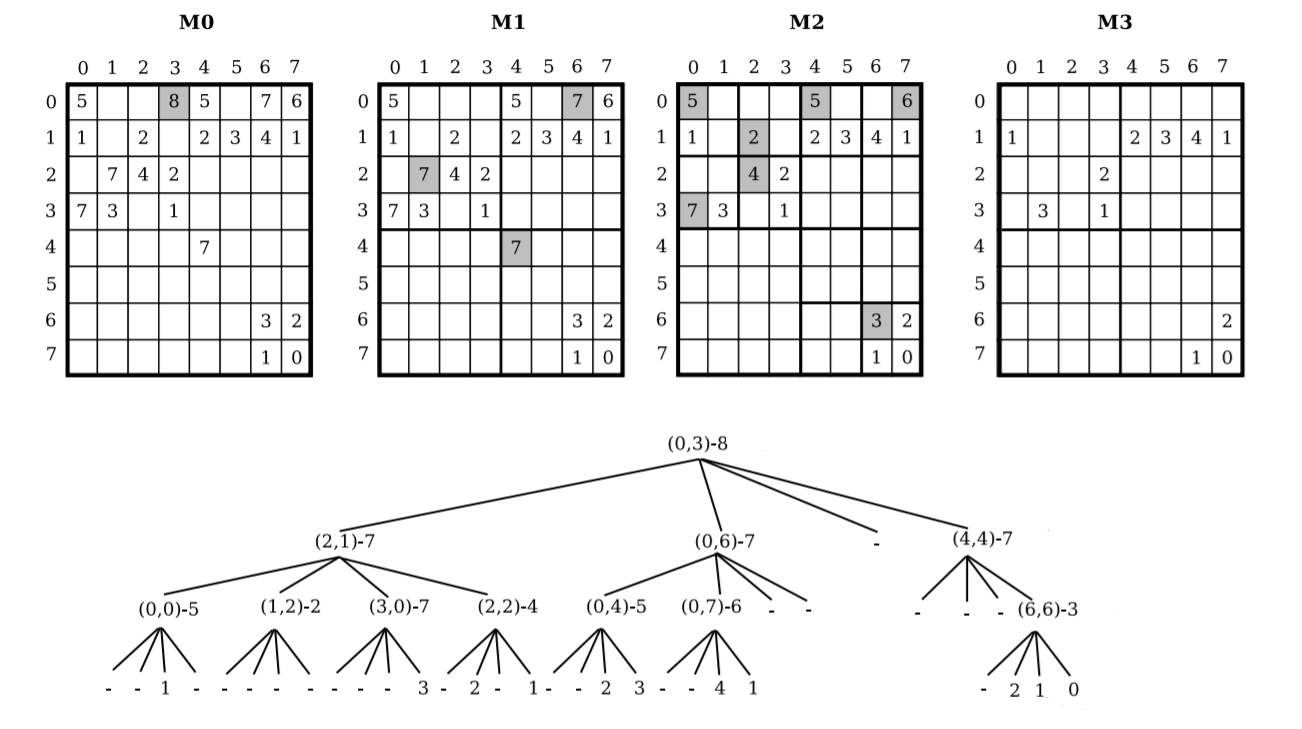
\includegraphics[height=200 pt, width=380 pt]{./ressources/image/k2-treaps.png} 
\end{center}
\caption{Exemple d'une représentation $k^2$-treap d'un graphe pondéré}
\label{k2-treaps}
\end{figure}

Pour avoir une bonne compression, $k^2$-treap effectue des transformations sur les données stockées. La première transformation consiste à changer les coordonnées représentées dans l'arbre en des coordonnées relatives par rapport à la sous matrice actuelle. La deuxième est de remplacer chaque poids dans l'arbre par la différence entre sa valeur et celle de son parent.\\
Trois structures de données sont utilisées pour sauvegarder les coordonnées et les valeurs des cellules ainsi que la topologie de l'arbre. Chaque structure est détaillée dans ce qui suit :
\begin{itemize}
\item \textit{Listes de coordonnées locales :} La séquence de coordonnées de chaque niveau \textit{l} de l'arbre est stockée dans une liste \textit{coord}[\textit{l}].
\item \textit{Liste des valeurs : } Le parcours de l'arbre se fait en largeur, la séquence des valeurs récupérées est stockée dans une liste nommée \textit{values}. Un tableau nommé \textit{first} est utilisé pour sauvegarder la position début de chaque niveau dans \textit{values}.
\item \textit{L'arbre :} La structure de l'arbre $k^2$-treap est sauvegardée avec un arbre $k^2$-tree, les nœuds contenant des valeurs dans $k^2$-treap sont représentés par des uns et les nœuds vides par des zéros. Pour le stockage de l'arbre, un seul tableau T est utilisé. 
\end{itemize}

La figure \ref{k2-treaps-structure} représente les structures de données utilisées pour le stockage de l'arbre de la figure \ref{k2-treaps} précédente \citep{badr2013traitement} :

\begin{figure}[H]
\begin{center}
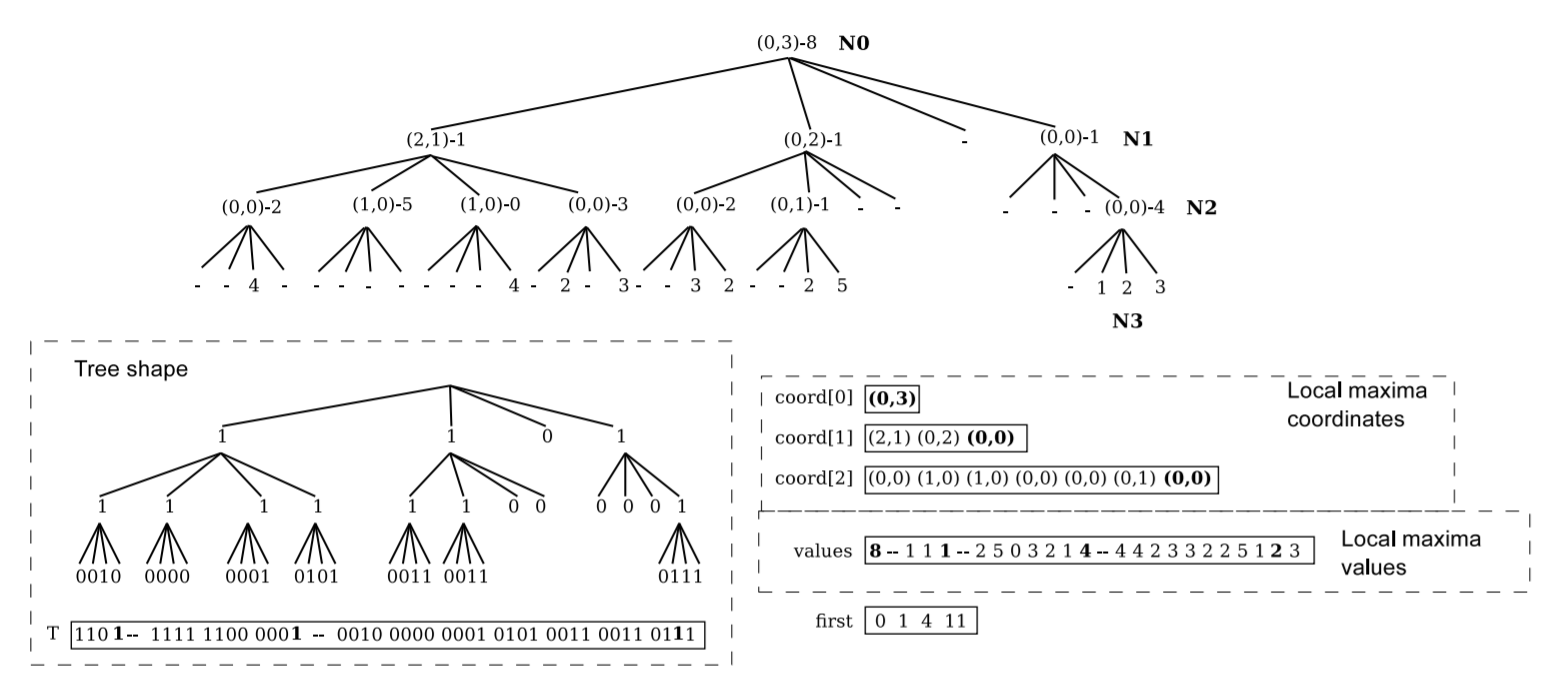
\includegraphics[height=200 pt, width=380 pt]{./ressources/image/k2-treaps-structure.png} 
\end{center}
\caption{Structures de données pour une représentation $k^2$-treap}
\label{k2-treaps-structure}
\end{figure}

%\subsubsection{I$k^2$-trees}
Garcia et al. \citep{garcia2014interleaved} proposent I$k^2$-tree pour Interleaved $k^2$-tree. Elle est appliquée sur les bases de données RDF ainsi que sur les graphes dynamiques. Dans les graphes dynamiques, les deux premières dimensions correspondent aux nœuds source et destination et la troisième dimension reflète le temps. Le graphe est donc défini par |T| matrices d'adjacence prisent à des instants $t_k$ différents. I$k^2$-tree représente les matrices simultanément. Chaque matrice est représentée par un arbre $k^2$-tree et ils sont par la suite regroupés dans un seul arbre. Chaque nœud de l'arbre obtenu représente une sous-matrice comme dans l'algorithme de base, sauf qu'au lieu d'utiliser un seul bit, I$k^2$-tree utilise 1 à |T| bits pour représenter le nœud. Le nœud racine contient |T| bits. Le nombre de bits de chaque fils dépend du nombre de uns de son parent. L'arbre finale est toujours stocké avec deux tableaux : T et L.
La figure \ref{Ik2-trees} est un exemple de I$k^2$-tree appliqué sur un graphe dynamique représenté dans trois instants \citep{garcia2014interleaved} :

\begin{figure}[H]
\begin{center}
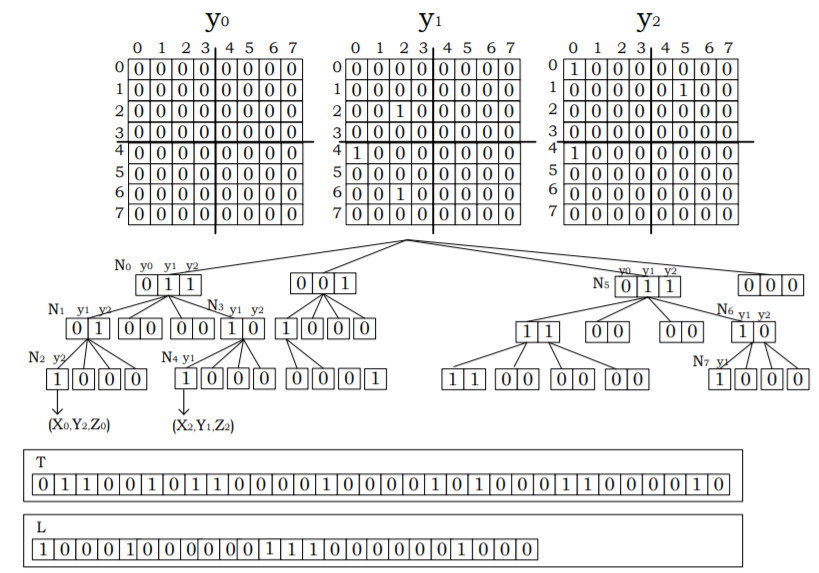
\includegraphics[scale=0.55]{./ressources/image/Ik2-trees.png} 
\end{center}
\caption{Exemple d'une représentation I$k^2$-tree}
\label{Ik2-trees}
\end{figure}

%\subsubsection{diff I$k^2$-trees}
Une variante de I$k^2$-tree appelée Differential I$k^2$-tree a été étudiée dans \citep{alvarez2017succinct}. Elle vise à améliorer le taux de compression en représentant uniquement les changements survenus sur le graphe à un instant $t_i$ au lieu d'une instance complète : à l'instant $t_0$, une capture complète du graphe (matrice d'adjacence) est stockée. À l 'instant $t_k$, pour k>0, seules les arrêtes qui changent de valeurs entre $t_{k-1}$ et $t_k$ sont stockées. Les matrices sont représentées à la fin de la même manière que I$k^2$-tree. La limite de cette représentation est que la structure doit être décompressée lors d'une requête.
La figure \ref{Ik2-trees-diff} montre un exemple d'une représentation diffI$k^2$-trees \citep{alvarez2017succinct}.

\begin{figure}[H]
\begin{center}
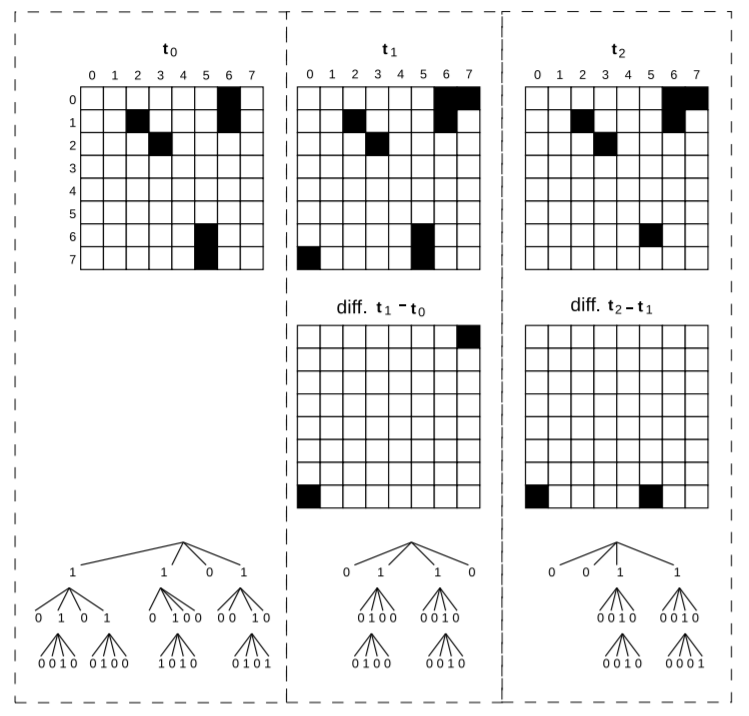
\includegraphics[scale=0.8]{./ressources/image/Ik2-trees-diff.png} 
\end{center}
\caption{Exemple d'une représentation diff I$k^2$-tree}
\label{Ik2-trees-diff}
\end{figure}

%\subsubsection{Att $K^2$-trees }
Dans \citep{alvarez2018compact}, les auteurs étendent la représentation $k^2$-tree pour les bases de données orientées graphes. Ces graphes sont étiquetés, attribués, orientés et ont des arêtes multiples. Ils présentent le graphe sous forme d'une nouvelle structure intitulée Att$k^2$-tree pour Attributed $k^2$-trees.
La figure \ref{k2-trees-att-graphe} montre un exemple de graphe pris en compte par Att$K^2$-tree \citep{alvarez2018compact}.

\begin{figure}[H]
\begin{center}
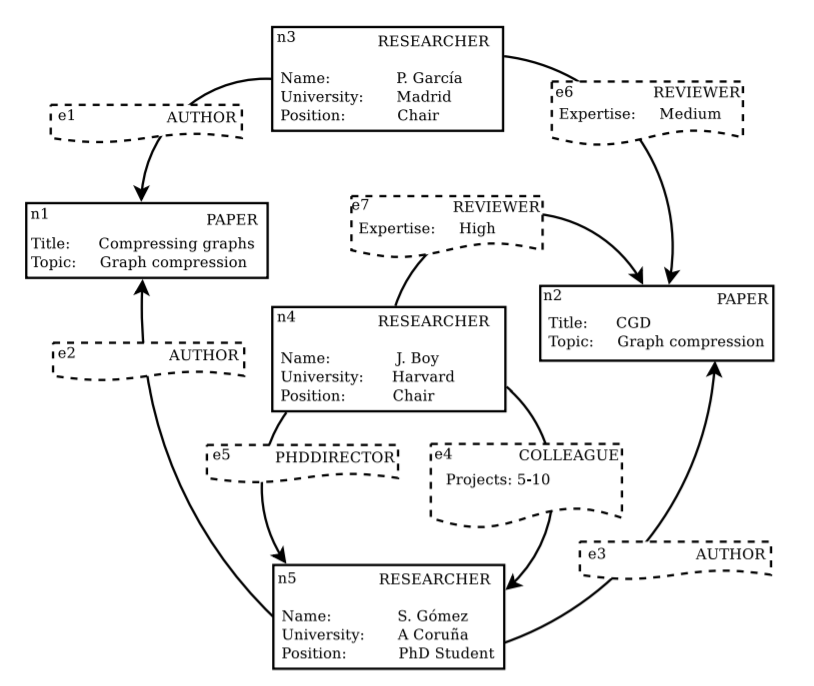
\includegraphics[height=200 pt, width=280 pt]{./ressources/image/k2-trees-att-graphe.png} 
\end{center}
\caption{Exemple d'un graphe étiqueté, attribué, orienté et multiple}
\label{k2-trees-att-graphe}
\end{figure}

\textbf{Structures de données :} La représentation obtenue par la compression est composée d'un ensemble d'arbres $k^2$-tree et d'autres structures supplémentaires. Le graphe est représenté par trois composantes: un schéma de données, les données incluses dans les nœuds et les liens et finalement la relation entre les éléments du graphe. Chaque composant est présenté dans ce qui suit :
\begin{itemize}
\item \textit{Schéma : } Ce composant gère les étiquettes et les attributs de chaque type d'éléments, il joue le rôle d'un index dans la représentation. Il est composé de :
\begin{description}
\item[Un schéma de nœuds :] représenté par un tableau qui contient les étiquettes des nœuds ordonnées lexicographiquement. Un identifiant est attribué à chaque nœud du graphe selon l'ordre du tableau, les \textit{$m_1$} nœuds possédant la première étiquette du tableau vont avoir des identifiants de 1 à \textit{$m_1$}, les \textit{$m_2$} nœuds avec la deuxième étiquette du tableau vont avoir des identifiants de \textit{$m_1$}+1 à \textit{$m_1$}+\textit{$m_2$} et ainsi de suite. Chaque entrée du tableau va ainsi stocker le plus grand identifiant portant son étiquette, cela permet de trouver l'étiquette d'un nœud à travers son identifiant.
\item[Un schéma d'arêtes :] Comme dans le cas des nœuds, un tableau est utilisé pour stocker les étiquettes des arêtes avec le même principe.  
\end{description}
Le schéma est le point de départ de la représentation, il permet d'obtenir l'étiquette d'un nœud ou d'une arête, et d'accéder à ses attributs.
\item \textit{Données :} Ce composant contient toutes les valeurs que peut prendre un attribut dans le graphe. Un attribut peut être représenté de deux façons différentes selon sa fréquence d'apparition, on distingue donc deux types d'attributs :
\begin{description}
\item[Attributs rares :] Ce sont les attributs qui prennent généralement des valeurs différentes à chaque apparition, ils sont stockés dans des listes et indexés avec l'identifiant de l'élément.
\item[Attributs fréquents :] Ce type d'attributs est sauvegardé dans deux matrices, une pour les attributs des nœuds et l'autre pour les attributs des liens. Les matrices sont stockées sous forme d'arbres $k^2$-trees.
\end{description}
La figure \ref{k2-trees-att-schema} illustre les deux composants schéma et données de la représentation Att$k^2$-trees  de la figure \ref{k2-trees-att-graphe} \citep{alvarez2018compact}:
\begin{figure}[H]
\begin{center}
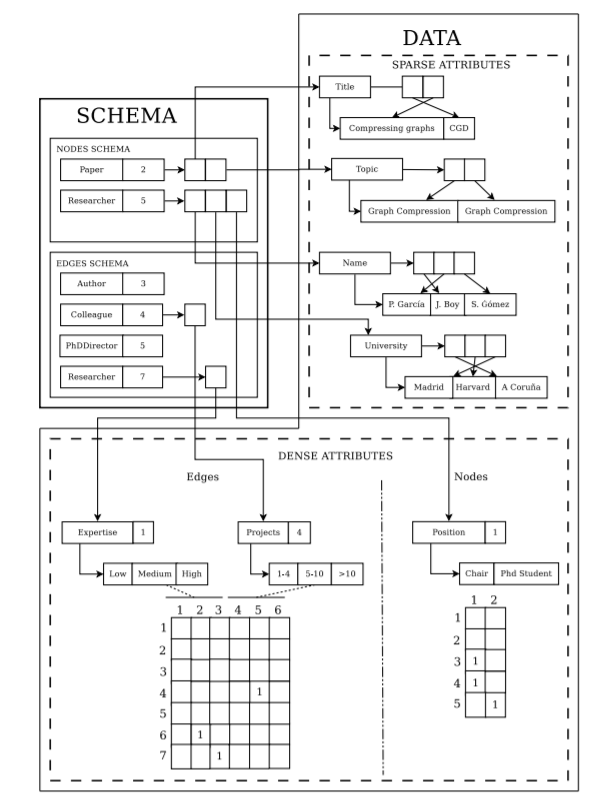
\includegraphics[scale=0.7]{./ressources/image/k2-trees-att-schema.png} 
\end{center}
\caption{Exemple d'une représentation Att$k^2$-tree (1/2)}
\label{k2-trees-att-schema}
\end{figure}


\item \textit{Relations :} C'est le dernier composant de Att$k^2$-tree, il stocke les relations entre les nœuds et les arêtes du graphe en utilisant un arbre $k^2$-tree et d'autres structures pour sauvegarder les identifiants des arêtes ainsi que les arêtes multiples. Les structures supplémentaires sont les suivantes :
\begin{description}
\item[Multi :] Un tableau qui indique si l'arête est multiple ou non.
\item[Firt :] Un tableau qui donne l'identifiant de l'arête, ou de celui de la première dans le cas d'une arrête multiple.
\item[Next :] Un tableau qui contient les identifiants des arêtes multiples restantes.
\end{description}
La figure \ref{k2-trees-att-relation} donne la représentation Att$k^2$-tree des relations du graphe de la figure \ref{k2-trees-att-graphe} \citep{alvarez2018compact}:
\begin{figure}[H]
\begin{center}
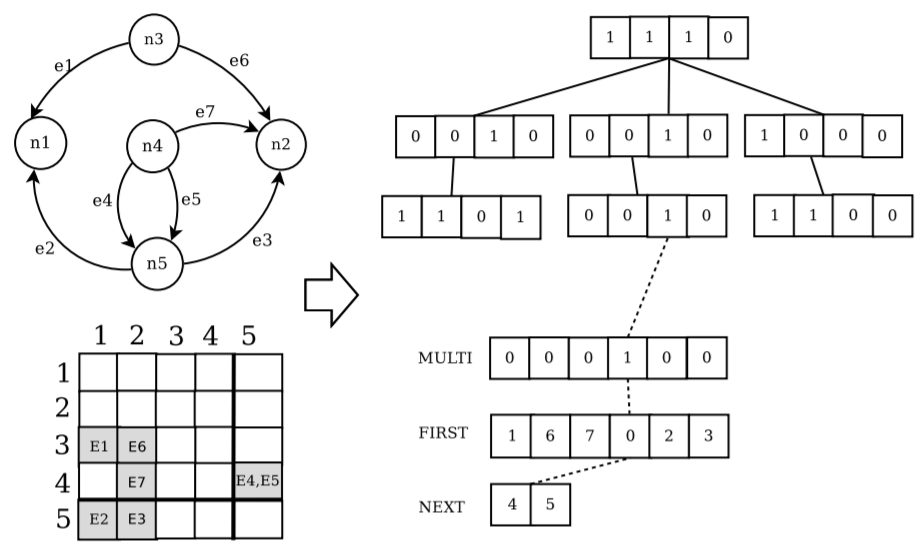
\includegraphics[height=200 pt, width=280 pt]{./ressources/image/k2-trees-att-relation.png} 
\end{center}
\caption{Exemple d'une la représentation Att$k^2$-tree (2/2)}
\label{k2-trees-att-relation}
\end{figure} 
\end{itemize}

%\subsubsection{dynAtt$k^2$-trees }
Dans le même article \citep{alvarez2018compact}, les auteurs étendent Att$k^2$-tree pour les graphes dynamiques. Ils proposent une nouvelle variante appelée dynAtt$k^2$-tree qui supporte le changement dans les attributs et les liens du graphe. Comme Att$k^2$-tree, dynAtt$k^2$-tree représente le graphe avec trois composantes : Schémas, données et relations. Les composantes sont semblables à ceux de Att$k^2$-tree mais avec certaines amélioration vue la nature dynamique du graphe.\\
\textbf{Structure de données : } 
\begin{itemize}
\item \textit{Schéma :}  En ce qui concerne les nœuds, leurs étiquettes sont stockées dans une liste dynamique ordonnée lexicographiquement. En outre, une séquence dynamique est utilisée pour sauvegarder le type de chaque nœud. Elle est stockée ensuite sous forme d'un arbre d'ondelettes \footnote{Ou wavelet en anglais, est un arbre binaire équilibré qui contient des données compressées dans une représentation optimale.} \citep{grossi2003high}. Le même principe est appliqué sur les arrêtes. 
\item \textit{Données :} Les attributs rares sont stockés dans des listes dynamiques, quant aux attributs fréquents, ils sont sauvegardés avec des arbres d$k^2$-trees (un arbre pour chaque attribut).
\item \textit{Relations :} Le stockage des relations se fait à l'aide d'un d$k^2$-tree et des tableaux dynamiques pour stocker les identifiants des arêtes et les arêtes multiples.
\end{itemize}




























